\documentclass[10pt]{article}
\usepackage[utf8]{inputenc}
\usepackage[a4paper, total={12cm, 22cm}]{geometry} % MARGIN 15.5 instead of 14 was initial

\usepackage{comment} 

\usepackage{hyperref}

\usepackage{float}
\usepackage{graphicx}

\usepackage[dvipsnames]{xcolor}
\usepackage[normalem]{ulem}

\setlength\parindent{0pt}
\setlength{\parskip}{2em}

\usepackage{amsmath}
\usepackage{listings}
\usepackage{comment}
\usepackage{longtable}
\usepackage{markdown}

\usepackage{biblatex}
\addbibresource{bibliography.bib}


% FOOTER AND HEADER %
\usepackage{etoolbox}
\usepackage{fancyhdr}
\pagestyle{fancy} 
\newcommand{\frontmatter}{\clearpage \cfoot{\thepage\ }
\fancyhead{}
\renewcommand{\headrulewidth}{0pt}
\setcounter{page}{1}
\pagenumbering{Roman}}
\newcommand{\mainmatter}{\clearpage \cfoot{\thepage\ of \pageref{LastPage}}
\fancyhead[LE,RO]{Group I}\fancyhead[RE,LO]{\leftmark}
\renewcommand{\headrulewidth}{0.4pt}
\setcounter{page}{1}
\pagenumbering{arabic}}
\newcommand{\backmatter}{\clearpage \cfoot{\thepage\ }
\fancyhead{}
\renewcommand{\headrulewidth}{0pt}
\setcounter{page}{1}
\pagenumbering{alph}}
\patchcmd{\chapter}{\thispagestyle{plain}}{\thispagestyle{fancy}}{}{}
% Front page background %
\usepackage[
firstpage=true,
opacity=0.25,
angle=0,
]{background}
\backgroundsetup{contents={
\includegraphics[scale=0.1]
{images/background.jpg}}}



\begin{document}

\begin{titlepage}
    \begin{center}
        \vspace*{1cm}

        \Huge
        \textbf{DevOps Exam Report}
        
        \vspace{0.5cm}
        
        \Large
        Group I
            
        \vspace{1.5cm}
         
        \textbf{Christian Skovsgaard Rieck (crie@itu.dk)}
        \textbf{Daniel Stokholm Thomsen (dant@itu.dk)}\\
        \textbf{Harpa Gudrún Hreinsdóttir (hahr@itu.dk)}
        \textbf{Johan Fritze Neve (jone@itu.dk)}
            
        \vspace{1.5cm}
        
       
            
        \vfill
            
        DevOps, Software Evolution and Software Maintenance\\
         KSDSESM1KU
            
        \vspace{0.8cm}
            
        
\includegraphics[width=0.4\textwidth]{images/ITU_logo_UK.jpg}
            
        \Large
        Department of Computer Science\\
        Denmark\\
        1st of June 2022
            
    \end{center}
\end{titlepage}

\frontmatter
\tableofcontents

\mainmatter

\section{System's perspective}
\subsection{Architecture and Design}
% Probably need package module view and c&c, especially the sequence diagram for interactions with subsystems
The system is a mini-version of Twitter, called MiniTwit.
The system has two main packages, a Blazor frontend and a ASP.NET core API. The API and Frontend decisions are described in detail in sections \ref{frontenddisc} \& \ref{apidisc}, respectively. The overall decision log can be found on \href{https://github.com/Arklaide/devopsITUproject/blob/main/report/sub-reports/decision_log.md}{our GitHub Repository}. See Fig. \ref{fig:package} for the package module view. The architectural views has been created based on the 3+1 model proposed by Christensen et al\cite{christensen20163+}.

\begin{figure} [H]
  \centering
  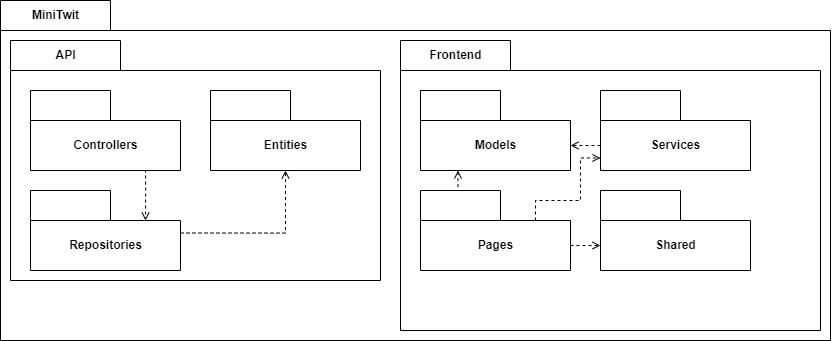
\includegraphics[width=0.9\textwidth]{images/devops-overall_module_view.png}
  \caption{Package diagram}
  \label{fig:package}
\end{figure}

The systems relies on various other services. The system uses ElasticSearch and Kibana for logging and Prometheus and Grafana for monitoring. The system is depicted in an overall context diagram in Fig. \ref{fig:context}. The six mentioned services are part of a docker stack swarm, which is managed by one docker swarm manager machine and supported by one docker swarm worker machine. The system, specifically the API, interacts with a managed database system. The database and the two machines are located and hosted in DigitalOcean.

\begin{figure} [H]
  \centering
  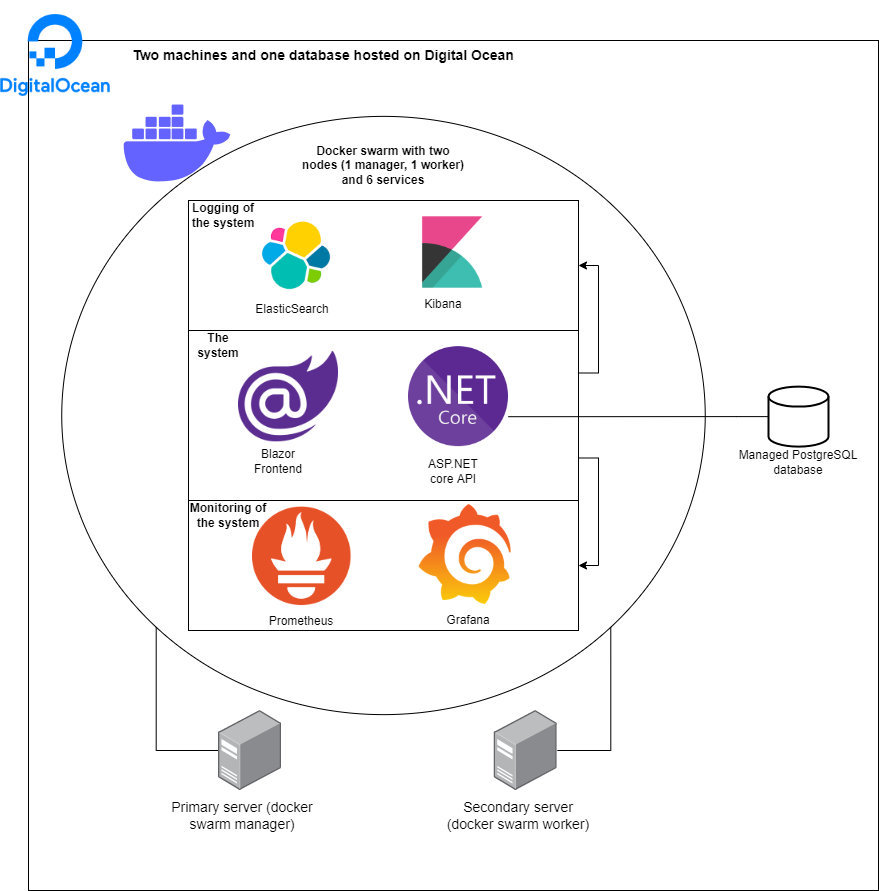
\includegraphics[width=0.9\textwidth]{images/devops-diagram.png}
  \caption{Context diagram}
  \label{fig:context}
\end{figure}

The Component \& Connector view can be seen in Fig. \ref{fig:cc}, which shows how the different components of the system are connected. The greyed out components are external, but are included to provide a better overview of how the system has been used in this project.

\begin{figure} [H]
  \centering
  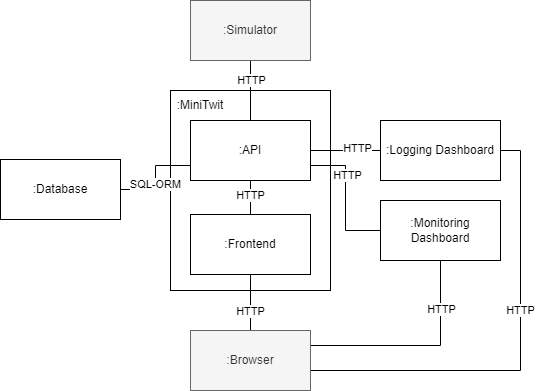
\includegraphics[width=0.9\textwidth]{images/devops-cc.png}
  \caption{Component \& Connector view}
  \label{fig:cc}
\end{figure}

An example of the interactions of subsystems can be seen on the sequence diagram in Fig. \ref{fig:sequence}. The example revolves around a user registration, and shows two scenarios, one where a user already exists and one where the user does not exists. The two scenarios returns different status codes and communicate differently with the logging and monitoring components.

\begin{figure} [H]
  \centering
  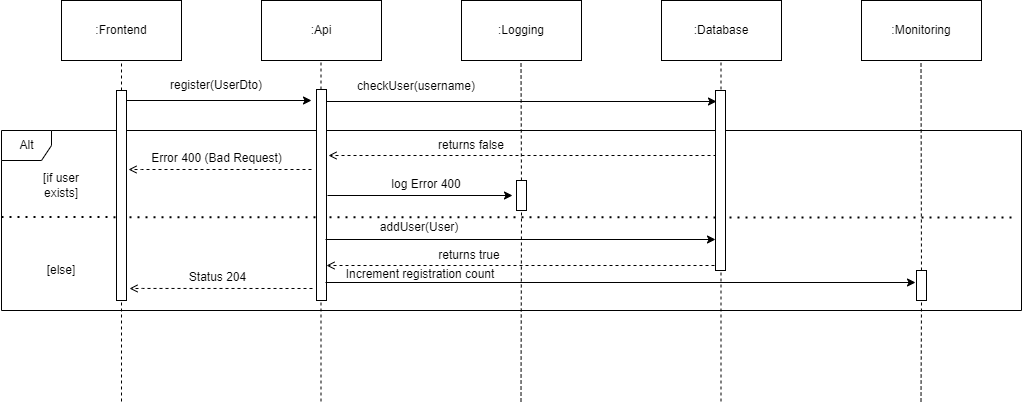
\includegraphics[width=0.9\textwidth]{images/devops-sequence.png}
  \caption{Sequence diagram}
  \label{fig:sequence}
\end{figure}

The deployment view of the system can be seen in Fig. \ref{fig:deloy}. The different entities are as follows:

\begin{itemize}
    \item \texttt{Digital Ocean Managed DB:} PostgreSQL database responsible for storing user data, following data and twits hosted on Digital Ocean. Kept separately from the servers to ensure backups and a less error prone environment for data storage.
    \item \texttt{Primary Server:} Ubuntu server responsible for managing the docker swarm.
    \begin{itemize}
        \item \texttt{API:} ASP.NET Core API responsible for communicating between the frontend and database acting as our backend.
        \item \texttt{Frontend:} Blazor frontend providing a user interface to view and create twits.
        \item \texttt{Prometheus:} Providing metrics for monitoring with default Prometheus metrics and custom metrics for the API.
        \item \texttt{Grafana:} Monitoring dashboard based on metrics from Prometheus to provide business and technical insight of the running system.
        \item \texttt{ElasticSearch:} Search for the aggregation of our logs sent from the API. 
        \item \texttt{Kibana:} A dashboard showing the logs with help from ElasticSearch.
    \end{itemize}
    \item \texttt{Secondary Server:} Ubuntu server responsible for being a docker swarm worker and hosting the docker instances requested by the manager.
\end{itemize}

\begin{figure} [H]
  \centering
  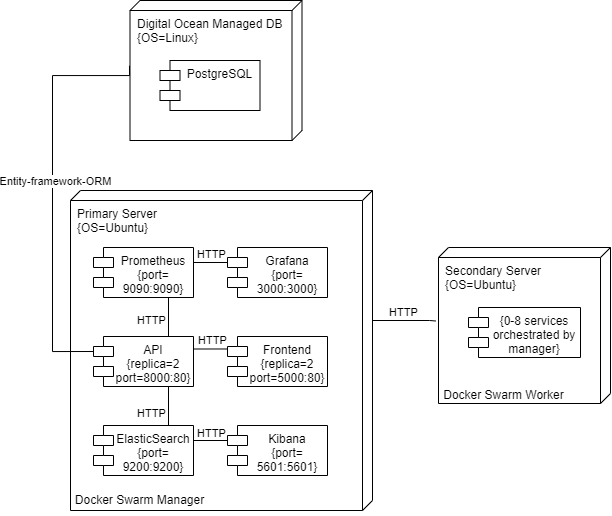
\includegraphics[width=0.9\textwidth]{images/devops-deployment.png}
  \caption{Deployment view}
  \label{fig:deloy}
\end{figure}

\subsubsection{Frontend}
\label{frontenddisc}

The frontend follows the model-view-controller pattern and uses .NET Core 5 with Blazor. 

The reasons why we decided to go with Blazor is based on the following factors:
\begin{enumerate}
\item The MVC pattern mixed with Blazor was chosen for the developers to easier understand the frontend setup as the API is structured mostly the same, without any views of course.
\item It is convenient to use the same language pack for both the frontend and API
\item Simple routing, httpClient and Dependency Injection
\end{enumerate}

To store the state of the logged in user we decided to go with a State class, which contains private functions to update authentication state. When the state is changed it notifies the dependant classes (which have injected the State class). 

To keep a clean structure we created a service layer where we store all calls to the API in an organized way. We use HttpClient to do the actual http call. 

\subsubsection{API}
\label{apidisc}
We have chosen to do the API using ASP.NET core 6 using controllers and the repository pattern. There are several reasons for why we chose this stack:
\begin{enumerate}
    \item Endpoints are automatically serialized to properly formatted JSON, which is being used in our frontend, aswell as the simulator.
    \item URl-Routing is done inline easily, as well as query parameters and request bodies are automatically bound to method parameters
    \item Logging of database interactions are automatically added. When we setup the ELK-stack, we have to only do minor additions to have meaningful logging in our entire application.
    \item Entity Framework Core makes it easy to communicate with our database and is base for the repository architectural pattern choice.
\end{enumerate}
\subsection{Dependencies}
The direct dependencies of the API and frontend are visualized as a graph in Fig. \ref{fig:depgrapg}. The graph shows us that the API has 16 dependencies and the frontend has 7.
\begin{figure} [H]
  \centering
  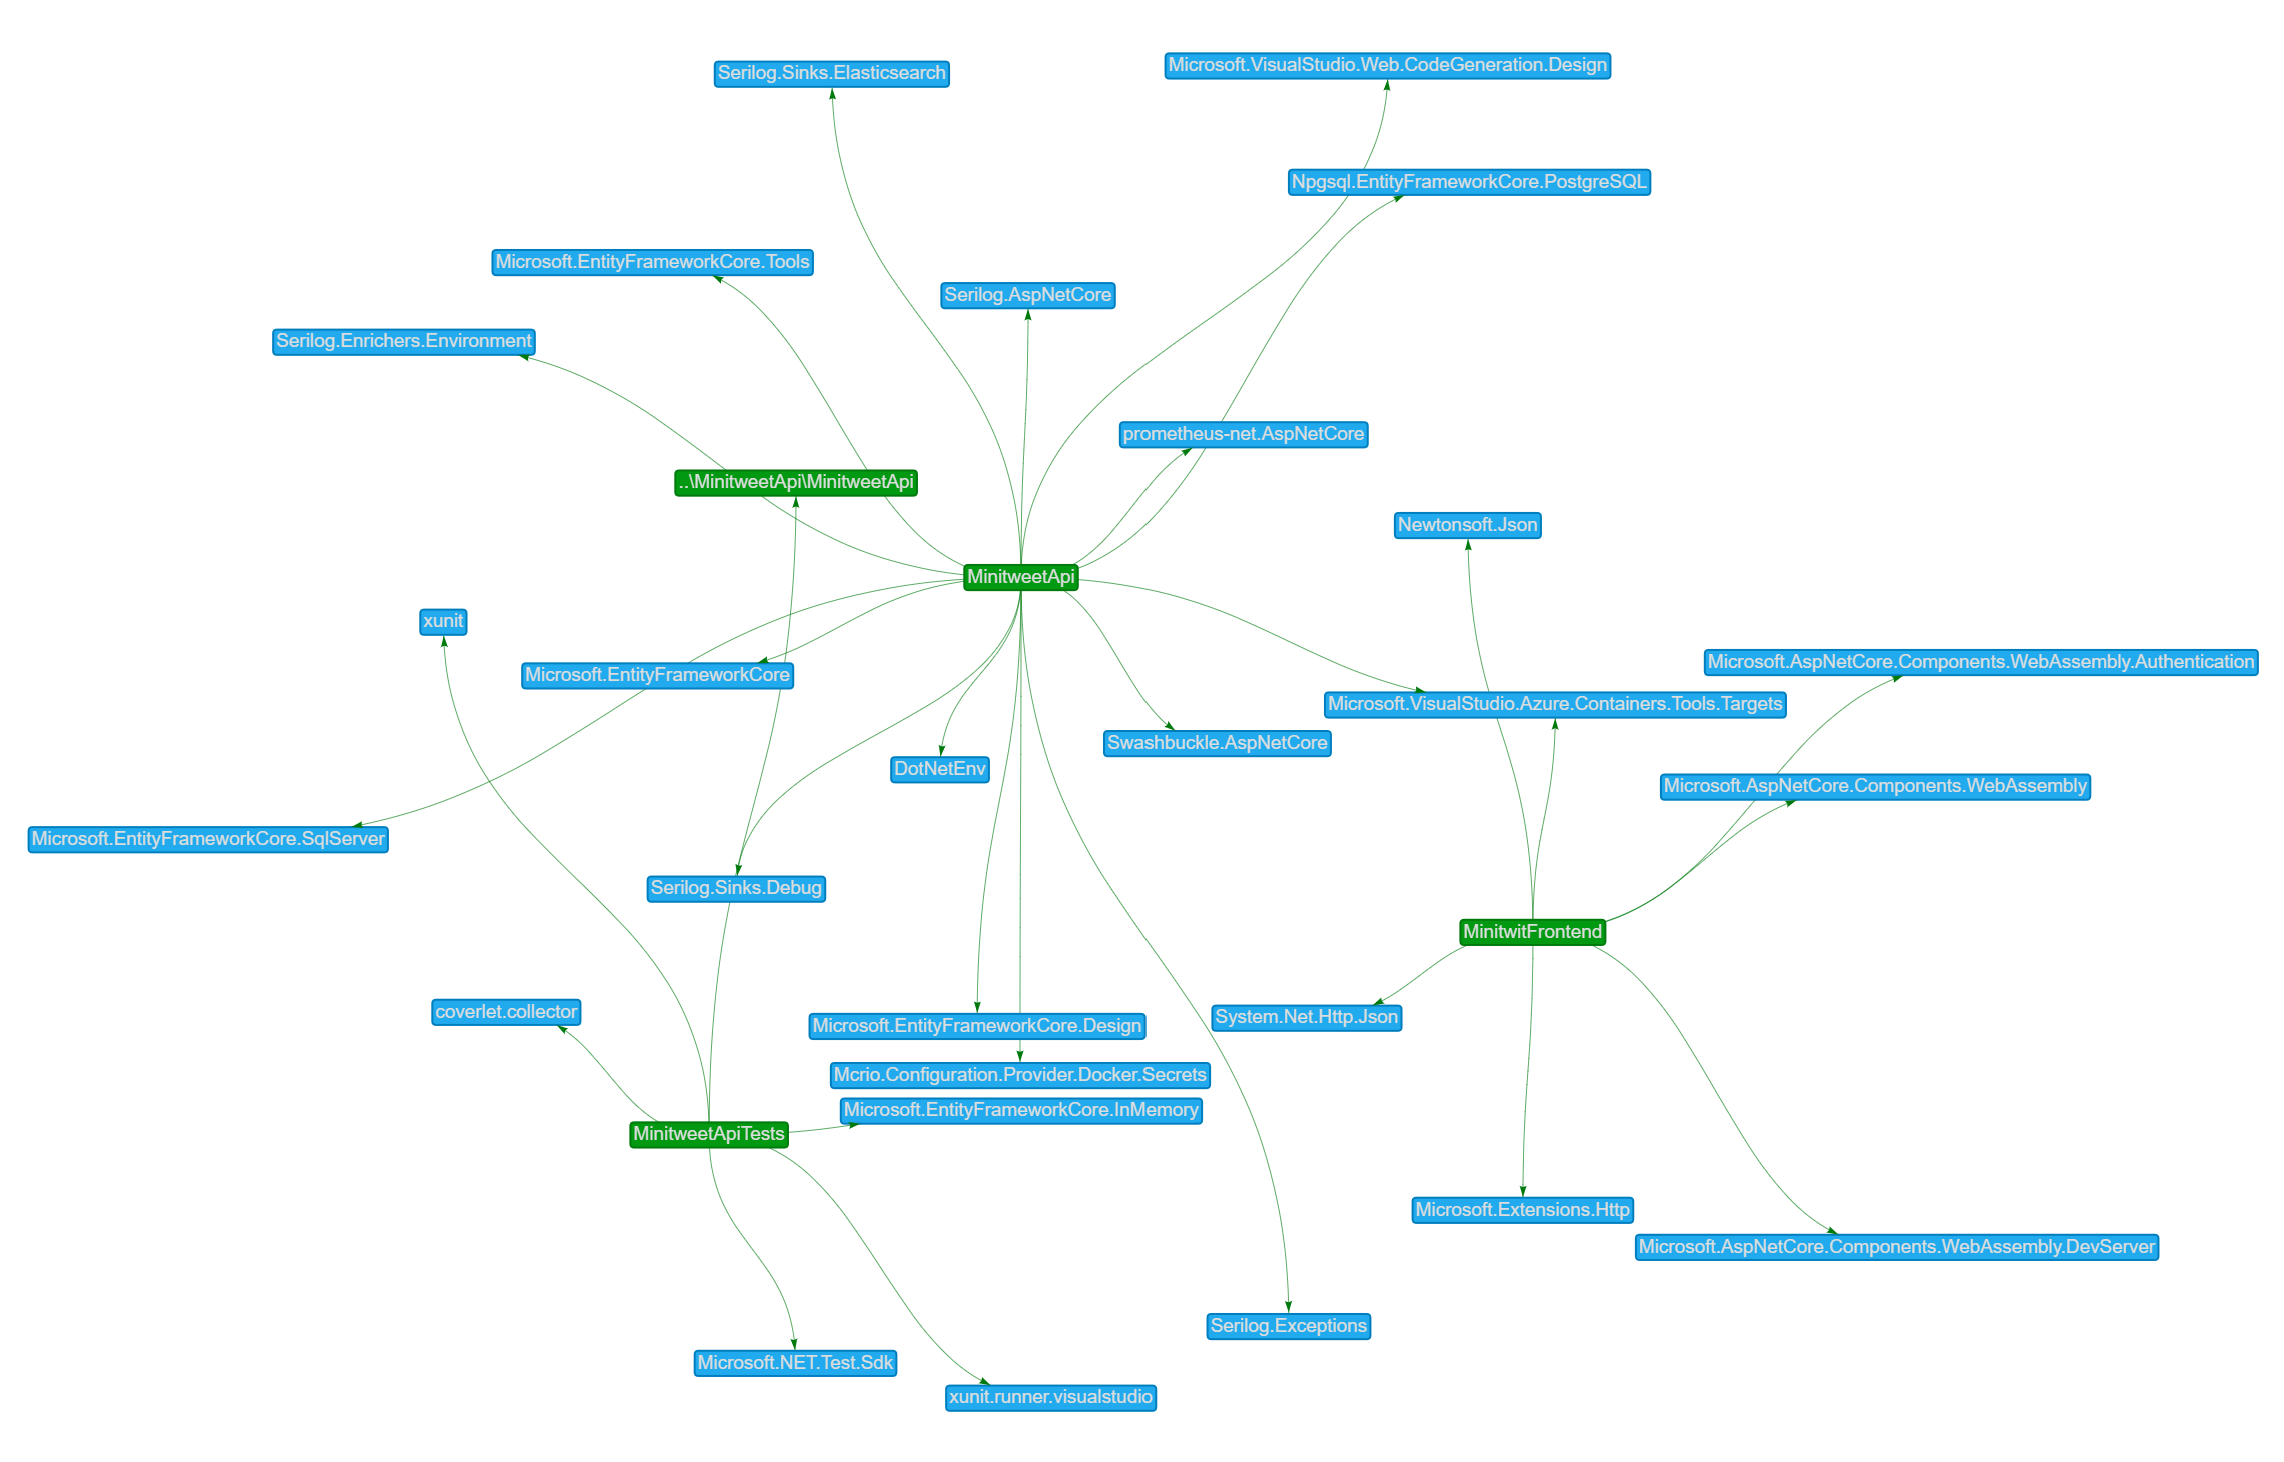
\includegraphics[width=0.9\textwidth]{images/dependencygraph.png}
  \caption{Dependency Graph}
  \label{fig:depgrapg}
\end{figure}

There are multiple other dependencies of the project, we depend on multiple GitHub actions in our workflows, such as SSH and checking code out. There are also dependencies in our docker images, such as nginx:alpine for the frontend image. Furthermore, our server other than standard Ubuntu dependencies, have docker.io \& doctl as dependencies. Lastly, we depend on Terraform for infrastructure as code. An overview can be seen in Fig. \ref{fig:otherdep}.

\begin{figure} [H]
  \centering
  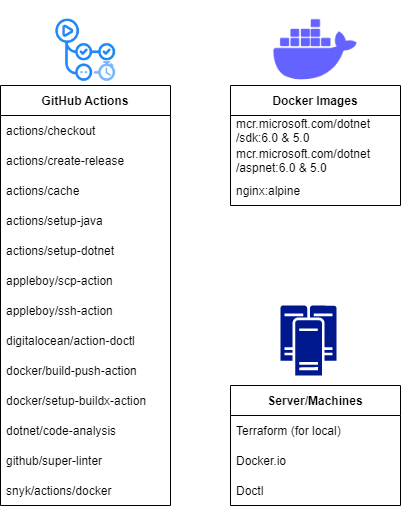
\includegraphics[width=0.7\textwidth]{images/devops-otherdependencies.png}
  \caption{Other dependencies overview}
  \label{fig:otherdep}
\end{figure}

An extensive list of all direct dependencies of this project, their name, description, and license can be found in appendix \ref{depappendix}.


\subsection{Current state of the systems}
The current state of the artifacts in the repository are summarized below, the state is found with different tools.
The state as analyzed by Better Code Hub can be seen in Fig. \ref{fig:bch}, it shows 8/10 checks looks good, however, automatic testing and short units of code are not passed. Another static analysis tool places our system in their category C, which means there is 10-20\% technical debt and they estimate it will take one week to clear out the debt. Moreover, the technical debt relates to 11 cases of code smells and 12 cases of code duplication. However, Sonar Cloud shows a better technical debt of less than 5\%, but a lower reliability score due to bugs. The Sonar Cloud state can be seen in Fig. \ref{fig:sc}. The overall state of the system is acceptable, but it opens up for various maintenance needs.

\begin{figure} [H]
  \centering
  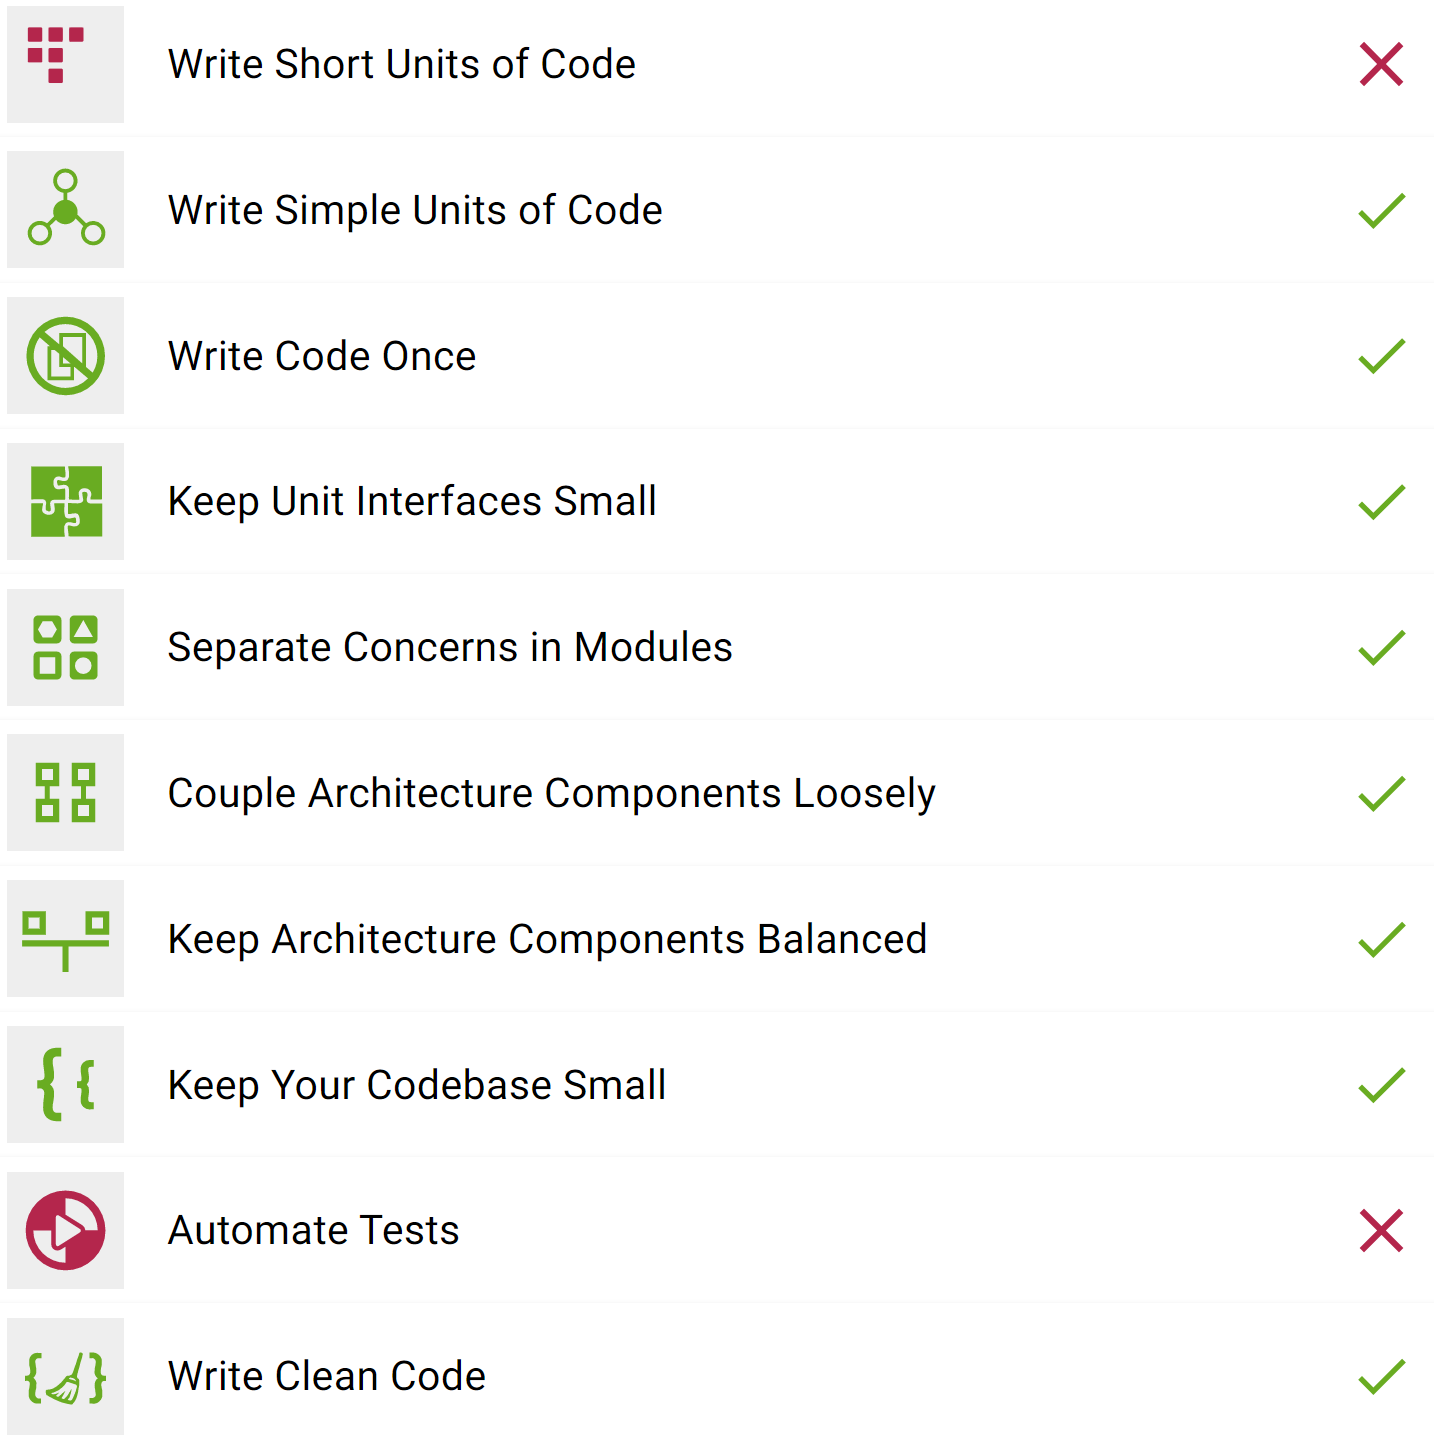
\includegraphics[width=0.9\textwidth]{images/bettercodehub.png}
  \caption{Better Code Hub state results}
  \label{fig:bch}
\end{figure}

\begin{figure} [H]
  \centering
  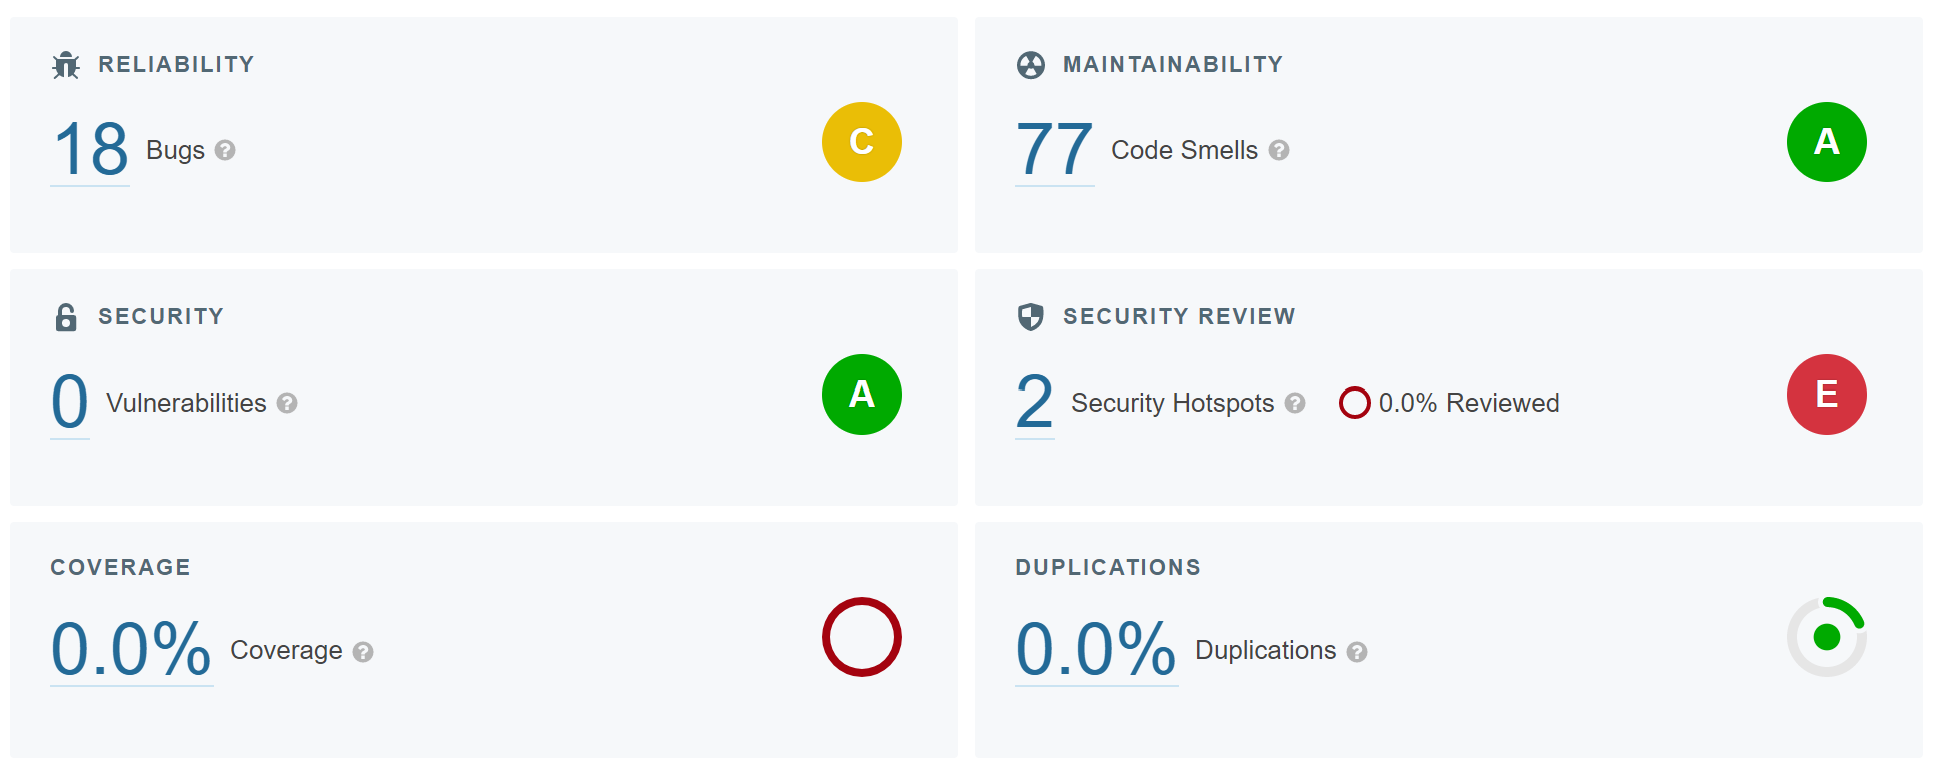
\includegraphics[width=0.9\textwidth]{images/sonarcloud.png}
  \caption{Sonar Cloud state results}
  \label{fig:sc}
\end{figure}


\subsection{Licenses}
We are using a MIT license which is a permissive, free, and open source license. All of our direct dependencies are using either MIT or Apache 2.0, which are both permissive licenses. That makes our MIT license compatible with all of our direct dependencies. \par
A typical software project often uses a lot of third-party packages so it can not always be easy to find all the licences. A tool which helped us to identify licenses is  \textbf{ScanCode}. However, due to issues with the output we were unable to identify all licenses thus we had to check all direct packages manually. 

\section{Process' perspective}
% Add general stuff think 3ways (+ contributions?)
% https://github.com/Arklaide/devopsITUproject/blob/main/report/sub-reports/ThreeWays.md
%How do you interact as developers?
%How is the team organized?
We have aimed to adhere to the "Three Ways" as described in "The DevOps HandBook\cite{kim2021devops}. A summary of our use of the three ways is described below, the initial internal notes concerning it can be found on our \href{https://github.com/Arklaide/devopsITUproject/blob/main/report/sub-reports/ThreeWays.md}{GitHub repository}.
\begin{itemize}
    \item \textbf{Flow:} A key task have been to simplify release to production in order to accommodate hot fixes and avoid big bang releases. We have a main branch for production and a develop branch for development/testing. Publishing to production narrows down to a pull request from develop to main that then triggers a deployment. The CI/CD pipeline is visualized in section \ref{cicdchain}. Furthermore, we keep track of our development process by using a Kanban board with columns representing the state of our issues. More details on the board in section \ref{Development_process}
    \item\textbf{Feedback and continual experimentation: }In the kickoff phase of the project we spend some time adjusting expectations and making sure that we each accommodate each other strengths and weaknesses. This is an important step to ensure mutual trust and a safe working environment where you are allowed to share failures, successes and ask for help. Openness provides a culture in which we all learn continuously and share experiences. Furthermore, we focus on continuously doing code reviews along with fast deployments allows us to secure and maintain good software quality.
\end{itemize}
%(basically a summary from these two files:%
%https://github.com/Arklaide/devopsITUproject/blob/main/report/sub-reports/ThreeWays.md%
%https://github.com/Arklaide/devopsITUproject/blob/main/report/sub-reports/contributions.md%
\subsection{Repository \& Branching strategy}
We chose to version control all our code as a mono-repository on GitHub. The repository can be viewed here: \href{https://github.com/Arklaide/devopsITUproject}{DevopsITUproject}.
There are two main folders/projects which has all the code that support our application:
\begin{enumerate}
    \item \href{https://github.com/Arklaide/devopsITUproject/tree/main/MinitweetApi}{MinitweetApi}
    \item \href{https://github.com/Arklaide/devopsITUproject/tree/main/MinitwitFrontend}{MinitwitFrontend}
\end{enumerate}
these projects are all in the same \href{https://github.com/Arklaide/devopsITUproject/blob/main/Minitweet.sln}{.sln} file, which is a way to structure projects in .NET.
We chose this option because we want to keep the number of repositories as low as possible, and also this makes our lives easier when working with the project since a change in the API often triggers some code changes to the Frontend and vice versa and therefore simpler to keep them in the same repository.
\\
\\
%Maybe a headline or some more text to explain this
All GitHub actions are stored in the same \href{https://github.com/Arklaide/devopsITUproject/tree/main/.github}{folder} for the sake of convenience.
\\
\\

%Maybe a headline or some more text to explain this
Some more significant parts of the repository are: %Delete this is it even neccesary?
\begin{enumerate}
    \item A docker-compose file for our production environment: \href{https://github.com/Arklaide/devopsITUproject/blob/main/docker-compose.production.yml}{docker-compose.production.yml}
    \item A license file: \href{https://github.com/Arklaide/devopsITUproject/blob/main/LICENSE}{LICENSE}
    \item \href{https://github.com/Arklaide/devopsITUproject/tree/main/Architecture-info}{.NET dependency graph}
\end{enumerate}

\subsubsection{Branching strategy}
We have been using the branching model known as GitFlow. This effectively means that we have a main branch for releases and a develop branch for development/testing. The workflow consists of the developer branching out from develop and after finishing their feature, they will do a pull request from their respective branch to the develop branch, where they have to assign at least one reviewer. When we are ready for a release, we create a PR from develop to main and once that is approved, our GitHub Action will automatically deploy the artifacts to DigitalOcean, and our newly improved system will be in production. A visualisation of the branching strategy in action can be seen here: \href{https://github.com/Arklaide/devopsITUproject/network}{Branch-visualized} 

\subsection{CI/CD chain}
\subsubsection{Releases}
To ensure we have a consistent form of GitHub releases, we have setup GitHub-actions that auto release. One of them just does a biweekly release and the other one does a release on pushes to the main branch. The GitHub actions can be found at the following links:
\begin{enumerate}
    \item \href{https://github.com/Arklaide/devopsITUproject/blob/main/.github/workflows/releaseonpush.yml}{Release on pushed to main}
    \item \href{https://github.com/Arklaide/devopsITUproject/blob/main/.github/workflows/autorelease.yml}{Biweekly release}
\end{enumerate}
\subsubsection{Pull Request}
To make sure that we have some consistency in our code before we push it to production we have added some GitHub checks that validate our code before merging pull requests, these are:
\begin{enumerate}
    \item The API and frontend is buildable and unit tests are run
    \item SonarCloud Code Analysis
    \item Better Code Hub
    \item Code Climate
    \item Snyk vulnerability scanning
\end{enumerate}
Taking a look at our release activity for the different weeks as seen in Fig. \ref{fig:release_activity}, it is  pretty easy to spot when we decided to add the auto release into our pipeline.
\begin{figure}[H]
    \centering
    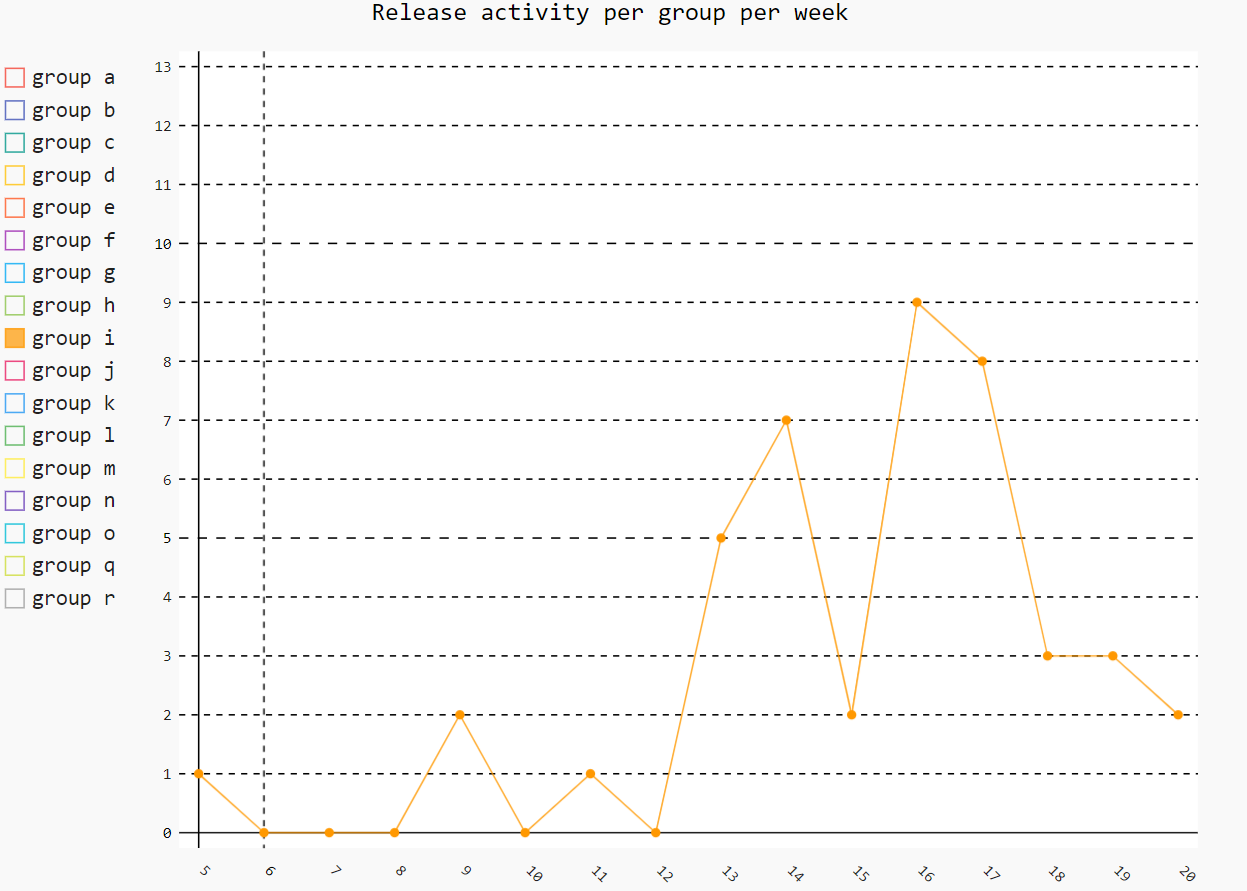
\includegraphics[width=\textwidth]{images/ReleaseActivity.PNG}
    \caption{Release activity}
    \label{fig:release_activity}
\end{figure}
\subsubsection{Deployment}
We have automated our deployment to production using a GitHub action: 
\href{https://github.com/Arklaide/devopsITUproject/blob/main/.github/workflows/deploy.yaml}{\textit{deploy action}}.
This action will trigger on every push to the main branch and will publish our system on our servers. 


\subsection{Development process}
\label{Development_process}
%Applied development process and tools supporting it
To have an overview of all issues and a platform to distribute and assign these, we have decided to use GitHub Project Board.
The board is divided into categories, and each issue is assigned one of the following categories:
\begin{enumerate}
    \item \texttt{Brainstorm/Ideas}: Where we keep track of new ideas.
    \item \texttt{Todo}: Where we keep our issues that needs to be done in the future
    \item \texttt{In Progress}: Here we keep our issues we are currently working on - We try to limit our work in progress to work in small batches to increase productivity. This also helps us in avoiding context switching, since we try to focus on one issue at the time.
    \item \texttt{Code review}: Here we keep our issues which are to be code reviewed before merging to the develop branch
    \item \texttt{Ready for release}: Here we keep our issues which are approved and waiting in develop to be merged for a release to main
    \item \texttt{Done}: Here we keep our issues which are done and deployed to main
\end{enumerate}
Each issue also has an assigned person. Combined with the status of the issues, we have a neat overview of open tasks.
\\
\\
The overview can be seen in Fig. \ref{fig:Kanban}


\begin{figure}[h]
    \centering
    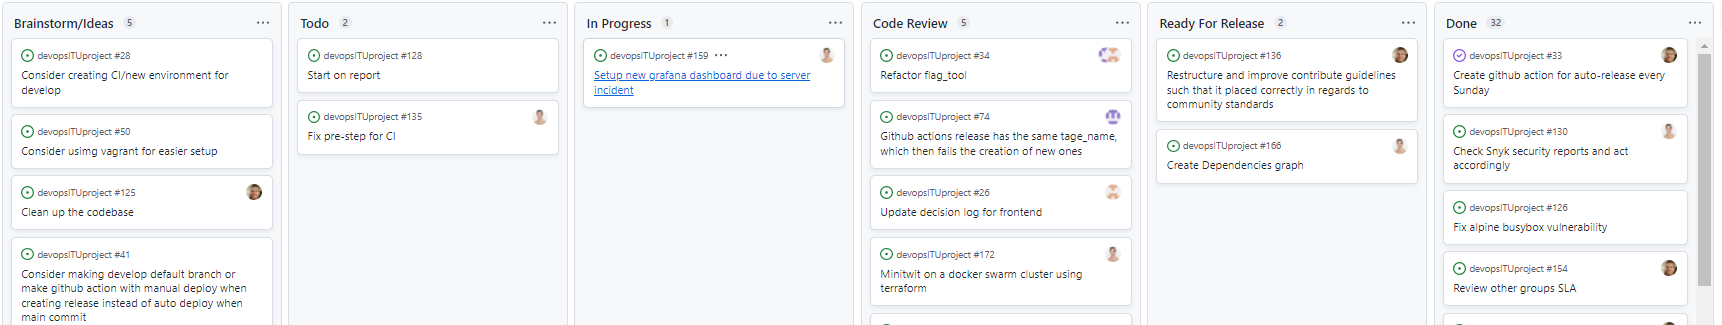
\includegraphics[width=\textwidth]{images/Kanban.PNG}
    \caption{Github Project Board}
    \label{fig:Kanban}
\end{figure}
\subsection{Flow of the CI/CD chain}
\label{cicdchain}
Fig. \ref{fig:flow} is a visualization of the entire process from a developers idea, to it being pushed to production.

\begin{figure}[H]
    \centering
    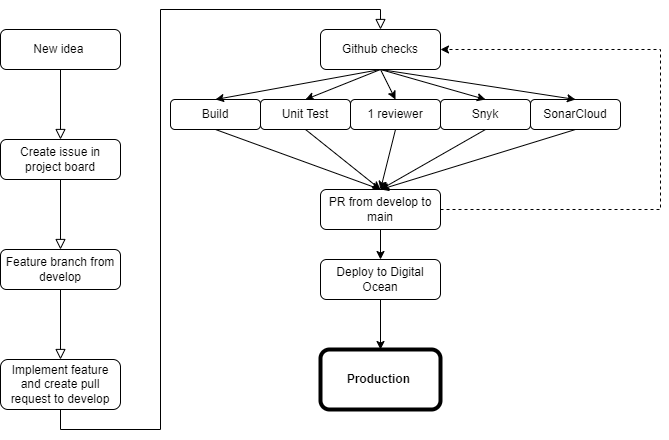
\includegraphics[width=\textwidth]{images/flow.PNG}
    \caption{CI/CD flow}
    \label{fig:flow}
\end{figure}


\subsection{Monitoring}
%How do you monitor (graphana/promitheus)
We are using Prometheus and Grafana as the monitoring platform for our application. There is a supported ASP.NET Core library for Prometheus so it is  easy for us to incorporate this into our system.
Inside our C\#-code we do the following to interact with prometheus:
\begin{enumerate}
    \item Have static readonly fields of the Metrics class, for metrics we want to monitor.
    \item Update the metrics using the prometheus API, when deemed fit.
\end{enumerate}

%What exactly do you monitor
We monitor several things in our system, for the business there are two important:
\begin{enumerate}
    \item The number of registered users since last release
    \item The number of times users have login to our system since last release 
\end{enumerate}
These are metrics which can be used by the business responsible to measure the growth and size of our application. Also having these two metrics, we can see if there are a lot of new users coming to our platform, or if its only the current users using our platform, given that we might have done some major updates to our system.

These metrics can be seen in Fig. \ref{fig:monitoring}. 
\\
\\
An example of how we use monitoring in our code can be seen here: \href{https://github.com/Arklaide/devopsITUproject/blob/main/MinitweetApi/Controllers/UsersController.cs}{\textit{Monitoring example}}.


\begin{figure}[h]
    \centering
    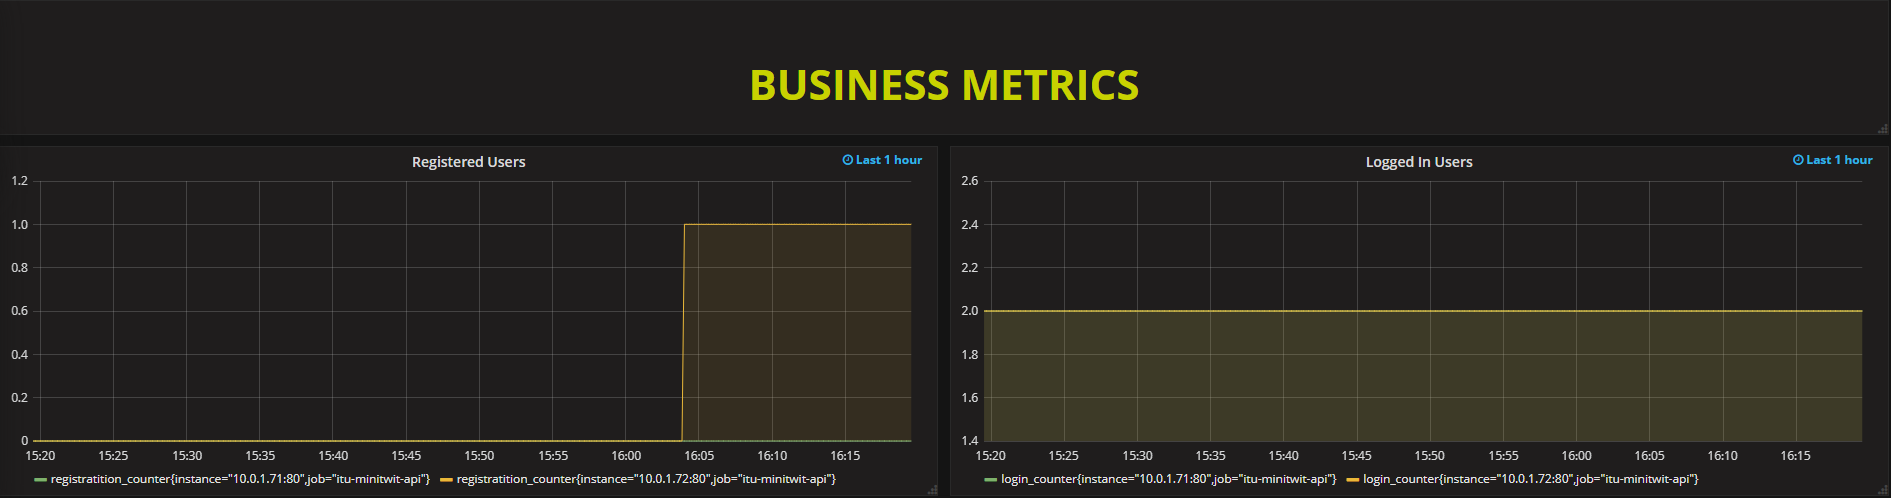
\includegraphics[width=\textwidth]{images/monitoringbusiness.PNG}
    \caption{Business metrics visualised from Grafana}
    \label{fig:monitoring}
\end{figure}
  
We also do some monitoring of the payload on our servers which gives us some valuable information of the servers performance.

Some of the things we deemed valuable are:
\begin{enumerate}
    \item The total user and system CPU time spent
    \item The amount of http requests to our application
    \item Total known allocated memory
\end{enumerate}

These are metrics that can give valuable information for a server engineer, to see the status of our servers and take decision, if we might need to apply vertical or horizontal scaling to our database or application server.

\begin{figure}[h]
    \centering
    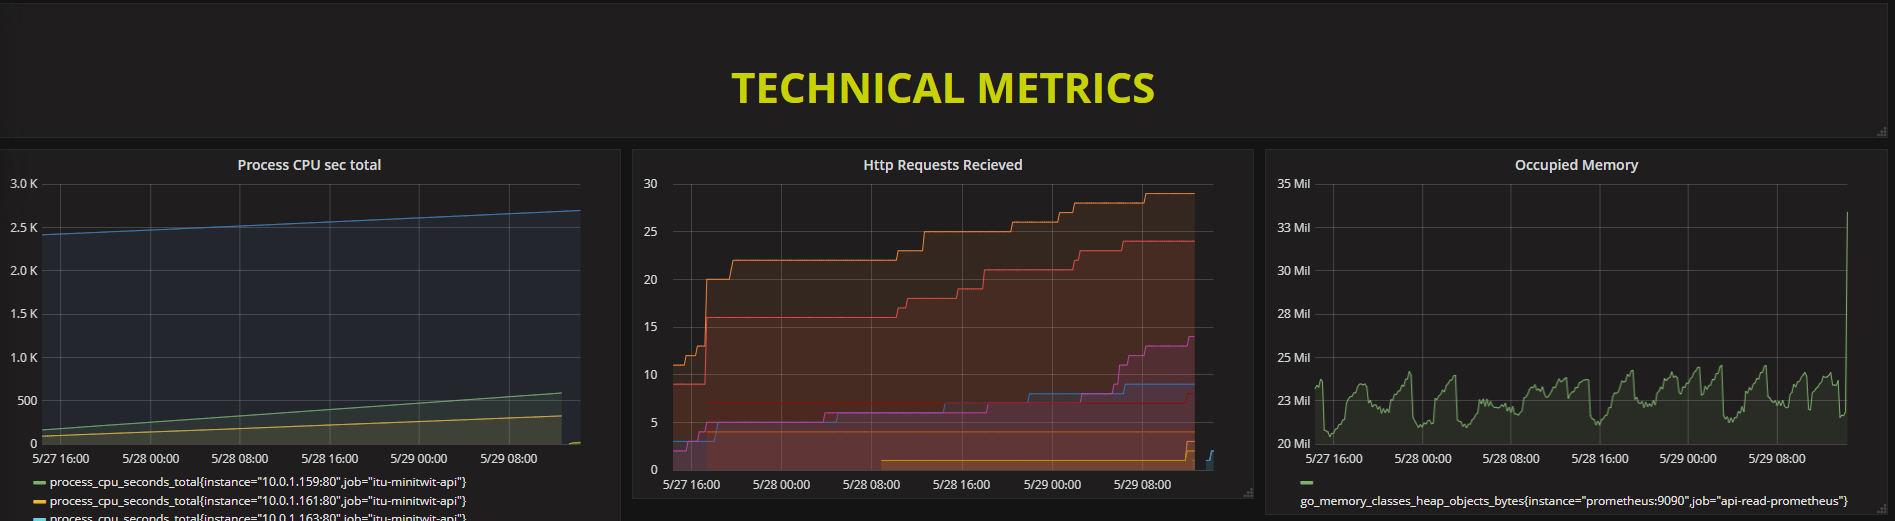
\includegraphics[width=\textwidth]{images/monitoring technical.PNG}
    \caption{Technical metrics visualised from Grafana}
    \label{fig:monitoringtechnical}
\end{figure}
Some more metrics that can give some valuable insights into our sytem can be seen here \href{https://github.com/Arklaide/devopsITUproject/blob/main/report/sub-reports/METRICS.md}{\textit{Metrics}} 

\subsection{Logging}
%motivation
To be able to better find failures in our application we have implemented logging, it is an essential part of troubleshooting, as it helps us keep a better track of all the interactions users have with our systems and thereby give us insights into problems that may arise as the system is being used by consumers.

%What do we log
We have decided to use the logging as is in Entity Framework 6. This means that every time our applications sends a command to the database, whether it being inserts, updates, or deletes, it is being logged. This means that all interactions with the API is being logged, and since the frontend mostly consist of API requests, we have a transitive logging relation to the frontend.    
%how do we aggregate logs
\\
\\
We have decided to use the popular ELK-stack which is a logging aggregation platform. First of all we use Serilog, which is a .NET logging library, to get all of our logging information sent to Elasticsearch. We then use Kibana to better query and visualize the data stored in the Elasticsearch database. We then have the possibility to filter the data on a lot of criteria which can give us good troubleshooting capabilities.

An example of the visualization of the logging can be seen in Fig. \ref{fig:logging_visualization}:
\begin{figure}[h]
    \centering
    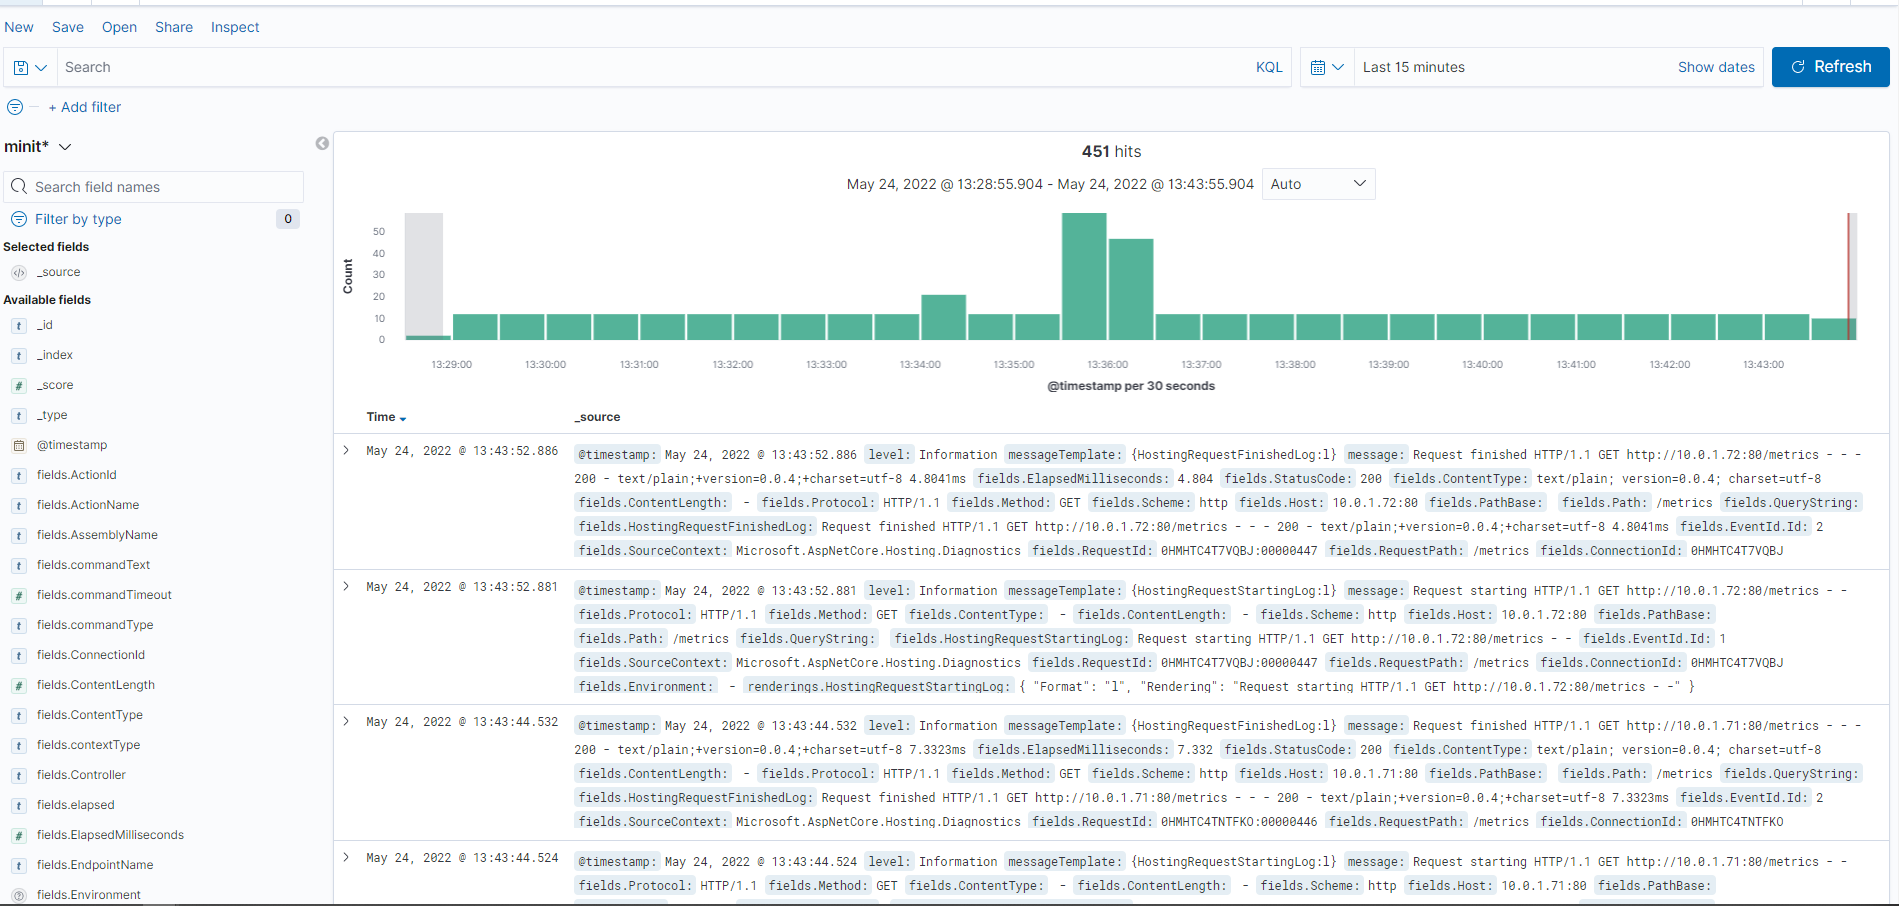
\includegraphics[width=\textwidth]{images/loggingvisualization.PNG}
    \caption{Logging visualization}
    \label{fig:logging_visualization}
\end{figure}
On the left hand side, we have all the fields which we can filter our logging data on.
On the top we can see a timeline of number of logs with time along the x-axis.

%This is perhaps to much and could be deleted, but describes the effectiveness of logging
In a hypothetical world where we would have customer support, a customer could contact us and tell us they had an error at a specific time. We would then be able to filter the error on time, and possibly on some other fields, (dependent on the error), and then we would have narrowed down the number of logs to a manageable level and, with these we would be able to figure out the problem and help out the costumer by resolving the issue. 
\subsection{Security assessment}
% passsword storage is not encrypted
% you don't need to type a password lol
The system has been assessed with regards to the security with two automatic penetration testing tools and a manual penetration testing. The whole security assessment report can be found in \href{https://github.com/Arklaide/devopsITUproject/blob/main/report/sub-reports/SecurityAssessment.md}{Our GitHub Repository}, this summary contains references found only there. The results are as following:

\begin{itemize}
    \item Metasploit WMAP on Kali has been run and it shows no vulnerabilities
    \item Skipfish on Kali has been run and it shows nothing important, but indicates missing charset
    \item The user info API endpoint sends the password in plain text (everyone can see this). This is broken access control, and relates to risk no 6.
    \begin{itemize}
        \item The hashing of the passwords seem broken
        \item It is possible to use this data to log in as other users
    \end{itemize}
\end{itemize}

The actions points based on the results are:
\begin{itemize}
    \item Implement counter measure for risk no 6
    \begin{itemize}
    \item Ensure proper salting, hashing and authentication 
    \item Ensure proper endpoint security
    \item Ensure no unnecessary data is sent as responses
    \end{itemize}
    \item Switch from HTTP to HTTPS for enhanced security
\end{itemize}

Furthermore, OWASP includes insufficient logging and monitoring as a security risk. The current state of our logging is acceptable, since it is possible to manual see some results from the penetration test, such as tools trying to access config sub-sites. However, nothing is automatic. Furthermore, the monitoring does not give much information, other than a few technical and business related metrics, such as numbers of logins. The security issue concerning risk no 6 that was found, can't be seen with the current logging/monitoring.

\subsection{Critical incident}
The group lost access to the first server of the project. It was no longer possible to log in via SSH-keys or in the DigitalOcean UI. The server was put in recovery mode, but access was still not possible to obtain even when resetting root password. The solution was to quickly deploy new servers, but now with two machines using Docker Swarm. The downtime was about 4 hours mostly due to creating a better setup with Docker Swarm and little manual configuration of the servers. It was not possible to find any suspicious activity, moreover, there was no extra load on CPU or other metrics of the server, which indicates that no one has installed a BitCoin miner or other types of software that needs server power. The root cause was never found, so the best corrective measure is to create the infrastructure as code. We now have support for Terraform, but this was not implemented on the time of the incident. The full incident report can be found on  \href{https://github.com/Arklaide/devopsITUproject/blob/main/report/sub-reports/incident_log.md}{our GitHub repository}.

\subsection{Scaling and load balancing}
The initial scaling was vertical since the logging service used up all the CPU. However, to avoid having a single point of failure, horizontal scaling was added via two machines and replicas for Docker containers.
The scaling and load balancing is set up with Docker Swarm. We have 6 Docker Services as a Docker Stack, two of them have two replicas, the API and frontend. The scaling is static with Docker Swarm and more replicas are not created during higher loads. The Docker Swarm has one manager and one worker node. The manager is responsible for load balancing with the default Ingress routing load balancer. However, having only one manager node is a single point of failure, and in real setup, there should be more managers and workers to ensure smooth operation. The deployment uses the Blue-Green strategy to ensure that new upgrade starts before the current one stops, and then it shifts the load to the new one when it is ready. However, it is important to note that the database is not included in this strategy, which could yield problems if there are migrations to the database in the update.

\section{Lessons Learned Perspective}
% Describe the biggest issues, how you solved them, and which are major lessons learned with regards to:

%evolution and refactoring
%operation, and
%maintenance
%of your ITU-MiniTwit systems. Link back to respective commit messages, issues, tickets, etc. to illustrate these.
%Also reflect and describe what was the "DevOps" style of your work. For example, what did you do differently to previous development projects and how did it work?



%In general
%General lessons learned from devops %
Lessons we learned from devops so far: 
\begin{itemize}
\item \textbf{Be open-minded} to try new software/packages/methods that already exist on the market.
\item Using a kanban board was very useful and specifically having a \textbf{very clear description} of what the task was about. In general keeping things organized and prioritizing the backlog was useful.

\item \textbf{Emphasize automation}. Building automation into the development life-cycle is critical to ensure that the software releases are consistent. Also, it allows the programmers to be liberated from less significant and time-consuming tasks to focus on processes that require more thinking and creativity.
\item \textbf{Using Docker in CI/CD}. Docker makes it easier to build and test the code in any environment to catch bugs early in the development life-cycle. Easy to scale.
\item \textbf{Security Testing}. Identifying threats to the system and measure potential vulnerabilities will minimize the risk of being hacked. We found it convenient to include the security testing in the CI so whenever there is some new code it runs a security scan on it before it gets released.
\end{itemize}



%evolution and refactoring
\subsection{Evolution and refactoring}
\textbf{Difficulties allowing the front-end to communicate with the API}\\ When we first tried to make the front-end communicate with our API endpoints we kept getting the error \textbf{'TypeError: Failed to fetch'}. This error did not give us a lot of information which made the process of figuring out why we kept getting this error a little slower. After a lot of playing around in the program.cs file in the API we found out that we needed to use CORS in order for the front-end to be able to use its endpoints. We had to specify which origins the API wanted to accept http requests from in the CORS settings. Since we specified the front-end origin there the API knew that http requests from that origin were not dangerous and finally let us through. 
%operation, and

\textbf{Get .NET 6/.NET 5 running on all the computers}\\ We ran into a few problems when downloading the correct .NET versions and getting the projects up and running on all the computers. Our biggest problem was with one MAC computer which did not allow us to create the initial API project in .NET 6 (even though it was downloaded on the machine). We ended up using a windows computer to do this step but in general Visual Studio was a poor IDE for the MAC computer and using Rider was much better.


\textbf{Refactoring the database using Object–relational mapping}\\
A lesson that we can take along with us is the fact that we can utilize a lot of support given by the programming languages and its associated framework and libraries. When we were first given the task to refactor the python code, we chose to do it using .NET (reasons described in \ref{apidisc}), here we were given the complete SQL schema, we could then have used the effective scaffolding of entity framework, to efficiently create all the model classes and the database context using the existing database.
\subsection{Operation}

\textbf{Importance of following separation of concerns when hosting on multiple servers}\\
One of the lessons we learned during the project, is the importance of separating concerns when writing code that is to be hosted on different servers. This really showed itself, when we had to implement logging.
We are using a logging library, Serilog, for logging and when we did the configuration of this we had to connect to the right Elasticsearch database, of course we had to make sure this worked in test before gong live with it in production, but since our test environment is different from our production, the ideal solution was to do the configuration in a higher level of abstraction, meaning that we never have to hard code IP's of the servers we are connecting to, this lead to a lot of commits which started with \href{https://github.com/Arklaide/devopsITUproject/commit/30149bd9f5b1696ac1e10e3e6806d8db11e16c26}{commit 30149bd} and ends with \href{https://github.com/Arklaide/devopsITUproject/commit/686ee3893fabcce450d1844bf1743780d690413a}{commit 686ee38}
The ticket relating to these commits can be seen here: \href{https://github.com/Arklaide/devopsITUproject/issues/61}{\textit{Add Logging to the System}}
Luckily this issues was resolved, but took a significant amount of time, which could have been spent more wisely.

\textbf{Difficulties testing operation and configuration leads to many fails and commits}\\
An important lesson concerned the configuration of automation of workflows, like the GitHub Action used to deploy the latest main branch to Digital Ocean. Operations and configuration is hard to test, the deploy action can only be tested by actually deploying to production. This had led to many small commits in order to adjust when the action failed. It would have been nice to have a similar setup for the develop branch, such that the configuration could be tested without affecting production. A develop environment was not prioritised due to the costs associated. An example is on the 14th of March, where there was around 20 consecutive commits to try and fix the deployment of the system. Everything from missing nginx in the docker image to serve the static contents of the Blazor frontend and including environment variables in the deploy action. It starts with \href{https://github.com/Arklaide/devopsITUproject/commit/3cd6a117458ed81d38d57dfeb5b15afc5e4b69f5}{commit 3cd6a11} and ends with \href{https://github.com/Arklaide/devopsITUproject/commit/11e7e21605977232ae87d0dc9dddf2ac9f25cb8f}{commit 109eb16}

%maintenance
\subsection{Maintenance}

\textbf{Cleaning old code to ensure a clean codebase}\\
An important part of maintenance is also optimizing old code. This also goes for our application. One of the thing that is in need of a cleaning is the file and folder structure of our code. As the application grows there are quite a big chance that the folder structure should evolve with it. However taking the time and effort to do so, should be of a higher prioritization than what we have done in the project.
However it is very difficult to find the time to go back and optimize when we have to stay ahead of the curve with the deadlines of the following week. 
These were addressed in the  \href{https://github.com/Arklaide/devopsITUproject/issues/125}{issue 125} this has sadly been lying dormant for a long time.
But for coming projects we clearly see the value of having a clean base to develop upon.

\section{Future work}
There are various artifacts of the system that could have an improved setup, these are, but are not limited to:
\begin{itemize}
    \item ElasticSearch hosted on its own machines to avoid the logs to be dependent on the same server as the API. Moreover, the heavy load of of ElasticSearch won't affect the other services.
    \item Better monitoring and logging to ensure better security and traceability. Especially alerts when something seem off.
    \item Add file change policy to CI/CD pipeline to avoid building unnecessary parts and speed up the process
    \item Enforce quality gates and check requirements both for pull requests and the deployment GitHub action to ensure overall quality
    \item Add an extra environment as Production but for the develop branch. An development/testing environment could help to avoid problems and coding/configuring in the dark. This, however, could slow the deployment, but ensure better quality assurance.
\end{itemize}

\label{LastPage}

\backmatter 
\printbibliography

\appendix
\section{Dependencies of the project}
\label{depappendix}
Below is a list of all the dependencies we are using in our project. Some of them have a strike-through which means we did not end up using them but they are currently still in our solution. One of the part of the maintenance phase is to get rid of dependencies that are not being used and we intend to do so in our solution as well.    


\end{document}